\documentclass[11pt,a4paper]{article}
\usepackage{fontspec}
\setmainfont{TeX Gyre Pagella}
\newfontfamily\headfont{Inter}[UprightFont=*-ExtraBold,BoldFont=*-ExtraBold,Extension=.otf,Path=/usr/share/fonts/opentype/inter/]
\usepackage[a4paper,margin=2.3cm]{geometry}
\usepackage{graphicx,booktabs,float,caption,array,xcolor}
\usepackage[hidelinks]{hyperref}
\usepackage{titlesec}
\usepackage[round]{natbib}
\usepackage{setspace}
\setstretch{1.05}
\renewcommand{\topfraction}{0.9}
\renewcommand{\bottomfraction}{0.8}
\renewcommand{\textfraction}{0.1}
\renewcommand{\floatpagefraction}{0.75}
\setlength{\parindent}{0pt}
\setlength{\parskip}{0.55em}
\titleformat{\section}{\headfont\Large}{\thesection}{0.8em}{}
\titleformat{\subsection}{\headfont\large}{\thesubsection}{0.8em}{}
\captionsetup{font=small,labelfont=bf}
\urlstyle{same}
\hypersetup{pdftitle={Ghost Towns of the World: Where Places Were Abandoned, and Why, in Open Data},pdfauthor={Tristan Hotham}}

\begin{document}
\begin{center}
{\Large\bfseries Ghost Towns of the World\par}
\vspace{0.4em}
{\large Where places were abandoned, and why, in Wikidata, Wikipedia\\and England's deserted medieval villages\par}
\vspace{1.2em}
{\large Tristan Hotham\par}
\vspace{0.3em}
{\small Independent researcher\\
ORCID: 0000-0003-4931-9349\\
DOI: \detokenize{10.5281/zenodo.23857616}\par}
\vspace{0.8em}
2026
\end{center}

\begin{quote}
\small
\begin{center}\textbf{Abstract}\end{center}
Ghost towns are abandoned for a handful of reasons: resources run out, wars and disasters strike, reservoirs flood valleys, nuclear accidents empty whole districts, and economies and populations drift away. I map the abandoned settlements recorded in open data and classify why each was abandoned. The sources are the 3,374 Wikidata items with coordinates classed as ghost towns, abandoned villages or deserted medieval villages, England's 2,074 deserted medieval villages and hamlets from Beresford's gazetteer, and the 492 places in English Wikipedia's `List of ghost towns by country'. Reasons come from transparent keyword rules applied to Wikidata descriptions and classes and to Wikipedia text, with a confidence for each. The main finding is about the record itself. 80\% of the Wikidata ghost towns are in the United States, and England's deserted villages make up 38\% of the 5,448 settlements mapped; Africa, Asia and South America together hold 34 Wikidata ghost towns. Only 165 Wikidata items (4.9\%) yield a reason, 61 of them from a mining word in the name alone. Wikipedia's list gives a reason for 300 of its places (61\%): mining and resource booms first (81), then war or military use (55) and natural disasters (54), economic decline (50), reservoirs (27) and nuclear accidents (24). Where a year is given, 85\% of abandonments fall after 1900, while England's dated deserted villages cluster in 1450 to 1699. The western United States has 1,053 ghost towns, 65 of them tied to mining, mostly by name. The data map who has catalogued abandonment as much as where it happened.

\textbf{Keywords:} ghost towns; abandoned settlements; deserted medieval villages; Wikidata; Wikipedia; mining; Chernobyl; open data bias
\end{quote}

\section{Introduction}
Settlements are abandoned when the reason for them disappears. T. Lindsey Baker's definition of a ghost town, ``a town for which the reason for being no longer exists'', is the one quoted at the head of Wikipedia's article on the subject \citep{wikighost}, and it points straight at causes. The article sorts them under a few headings: armed conflicts, economic decline, human intervention and infrastructure (including flooding by dams), and disasters, actual and anticipated. The reasons in this study follow those headings, split into seven: nuclear accident zones, war and military use, natural disasters and contamination, reservoirs, mining and resource booms, deserted medieval villages and plague, and economic decline, depopulation or relocation.

Scholars have studied particular kinds of abandonment in depth: the deserted medieval villages of England since \citet{beresford1954} and \citet{beresfordhurst1971}, the mining camps of the American West \citep{paul1963}, the towns emptied by Chernobyl. A world map that sets them side by side is harder, because no single source records abandoned places everywhere. Wikidata is the closest thing: an open, structured database with classes for ghost towns, abandoned villages and deserted medieval villages. This paper asks what it, with Wikipedia and one detailed national gazetteer, can say about where and why places were abandoned, and how far the answer reflects the record rather than history. An interactive map is at \url{https://maps.tristanhotham.com/ghost-towns/}.

\section{Data}
\textbf{Wikidata.} A query through QLever returned every item that is an instance of ghost town (Q74047), abandoned village (Q15661340) or deserted medieval village (Q1952852), or of a subclass of them, with its coordinates, English label, description, classes, country and any dissolution date: 19,444 rows for 10,217 items, of which 95 have no usable position. The subclass tree pulls in a great deal that is not a ghost town. 2,456 items are living Mexican municipalities, which reach the class through a faulty subclass link; 42 more are living towns, castles or museums. 4,249 are ancient cities and archaeological sites (Greek poleis, Roman towns, Iron Age oppida), 52\% of them in Turkey and Greece. I keep 3,374 items as ghost towns (Section~\ref{sec:methods}) and show the ancient sites as a separate layer, outside all counts.

\textbf{England's deserted medieval villages.} Beresford's Lost Villages, a digital edition of the gazetteer of \citet{beresfordhurst1971} published by the University of Hull, lists 2,074 deserted medieval villages and hamlets in England (2,000 villages, 74 hamlets), with positions, counties and, for 14 fully recorded counties, presumed dates of depopulation and written accounts. I use the version cleaned for an earlier study \citep{hotham2026lv}.

\textbf{Wikipedia.} English Wikipedia's `List of ghost towns by country' \citep{wikilist} gives 492 places in 90 countries and territories, usually with a sentence or two on what happened; the United States and Canada have their own lists and are not included. The article `Ghost town' \citep{wikighost} gives further examples, each linked to its own article.

\textbf{Geography.} Country, continent and first-level region (US state, Canadian province, English county) come from Natural Earth \citep{naturalearth}.

\begin{table}[tbp]\centering\small\caption{Sources and licences.}\label{tab:sources}
\begin{tabular}{>{\raggedright\arraybackslash}p{4.4cm}>{\raggedright\arraybackslash}p{6.8cm}>{\raggedright\arraybackslash}p{3.2cm}}\toprule Source & Used & Licence\\\midrule
Wikidata (via QLever) & Places, classes, descriptions, dissolution dates & CC0\\
Beresford's Lost Villages (University of Hull) & England's deserted medieval villages and hamlets, dates, causes mentioned & CC BY-NC-SA 4.0\\
English Wikipedia & `List of ghost towns by country', `Ghost town': reasons, years & CC BY-SA 4.0\\
Natural Earth & Countries, continents, states and provinces & Public domain\\
\bottomrule\end{tabular}\end{table}

\section{Methods}\label{sec:methods}
\subsection{Which items are ghost towns}
An item counts as a ghost town if one of its classes belongs to the ghost town family (ghost town, abandoned village, deserted medieval village, abandoned hamlet, former village, former town, mining community, pit village), or if it has a weaker class such as `former settlement' or `submerged settlement' and no ancient or archaeological class. Otherwise an item with an ancient or archaeological class goes to the ancient layer, and the rest are dropped. Items whose coordinates are given only as an unknown value are dropped. 1 Wikidata item that duplicated a site in Beresford's gazetteer (same name within 2 km) was removed. Deserted villages and hamlets are taken from Beresford's gazetteer; its shrunken, shifted, migrated and doubtful sites are left out.

\subsection{Reasons and confidence}
Each place gets one main reason from regular expressions, listed in full in the code (\texttt{reasons.py}) and on the interactive page. A text can match several reasons; the main one is the first in the order nuclear, war, disaster, reservoir, mining, medieval, economic, so that, for example, a mining town later drowned by a reservoir counts as a reservoir. Three kinds of text are searched: the place's entry in Wikipedia's list, including any sentence that introduces a group of entries (40 entries take their reason from such a sentence, for instance the villages of the Chernobyl zone); a sentence of the `Ghost town' article that links to the place; and the Wikidata description. Places within 45 km of the Chernobyl plant (covering Ukraine's 30 km zone and the Polesie reserve in Belarus) or 30 km of Fukushima Daiichi count as nuclear.

Confidence is \emph{high} when the reason is stated in words or comes from a zone, \emph{medium} when it follows from a Wikidata class alone (mining community, depopulated Palestinian village, deserted medieval village), and \emph{low} when it rests on a mining word in the place's name (Gold, Silver, Copper, Mine, Lode, Placer, Galena and others). Every deserted medieval village in Beresford's gazetteer counts as medieval with high confidence: the category is the reason, although the gazetteer's own accounts point to several causes.

Wikipedia entries were matched to Wikidata items when their names agreed after removing accents, case and qualifiers and the item lay in the entry's country; only unique matches were used (45 entries). Article sentences were matched in the same way (29), requiring the state or province to agree for titles such as `Centralia, Pennsylvania'. Most of the list's best-known places are absent from the Wikidata extract, because Wikidata classes them as towns or villages rather than ghost towns. So that the map can show them, I placed 44 of them by hand at approximate positions; they appear on the map but in no count.

\subsection{Dates}
Wikidata gives a dissolution date for 46 ghost towns. For Wikipedia entries I took the first year (or century, at its middle) at or after the first word of abandonment (abandoned, evacuated, flooded, destroyed and so on), which gives a year for 156 entries. England's dates are the gazetteer's presumed dates of depopulation, at the middle of each range, for the 270 sites with a usable date.

\section{Results}
\subsection{Where the record is}
Figure~\ref{fig:world} maps every place. Of the 3,374 Wikidata ghost towns, 2,700 (80\%) are in the United States, and 91\% of those have a formulaic one-line description (`ghost town in X County'), the sign of bulk entry. Canada has 265 (141 in Newfoundland and Labrador), Greece 101 and Australia 58; 41 of the 53 countries have fewer than ten (Figure~\ref{fig:countries}). Africa has 8, Asia 17 and South America 9. With England's 2,074 deserted villages added, England accounts for 38\% of the 5,448 settlements, and the United States and England together for 88\%.

\begin{figure}[tbp]\centering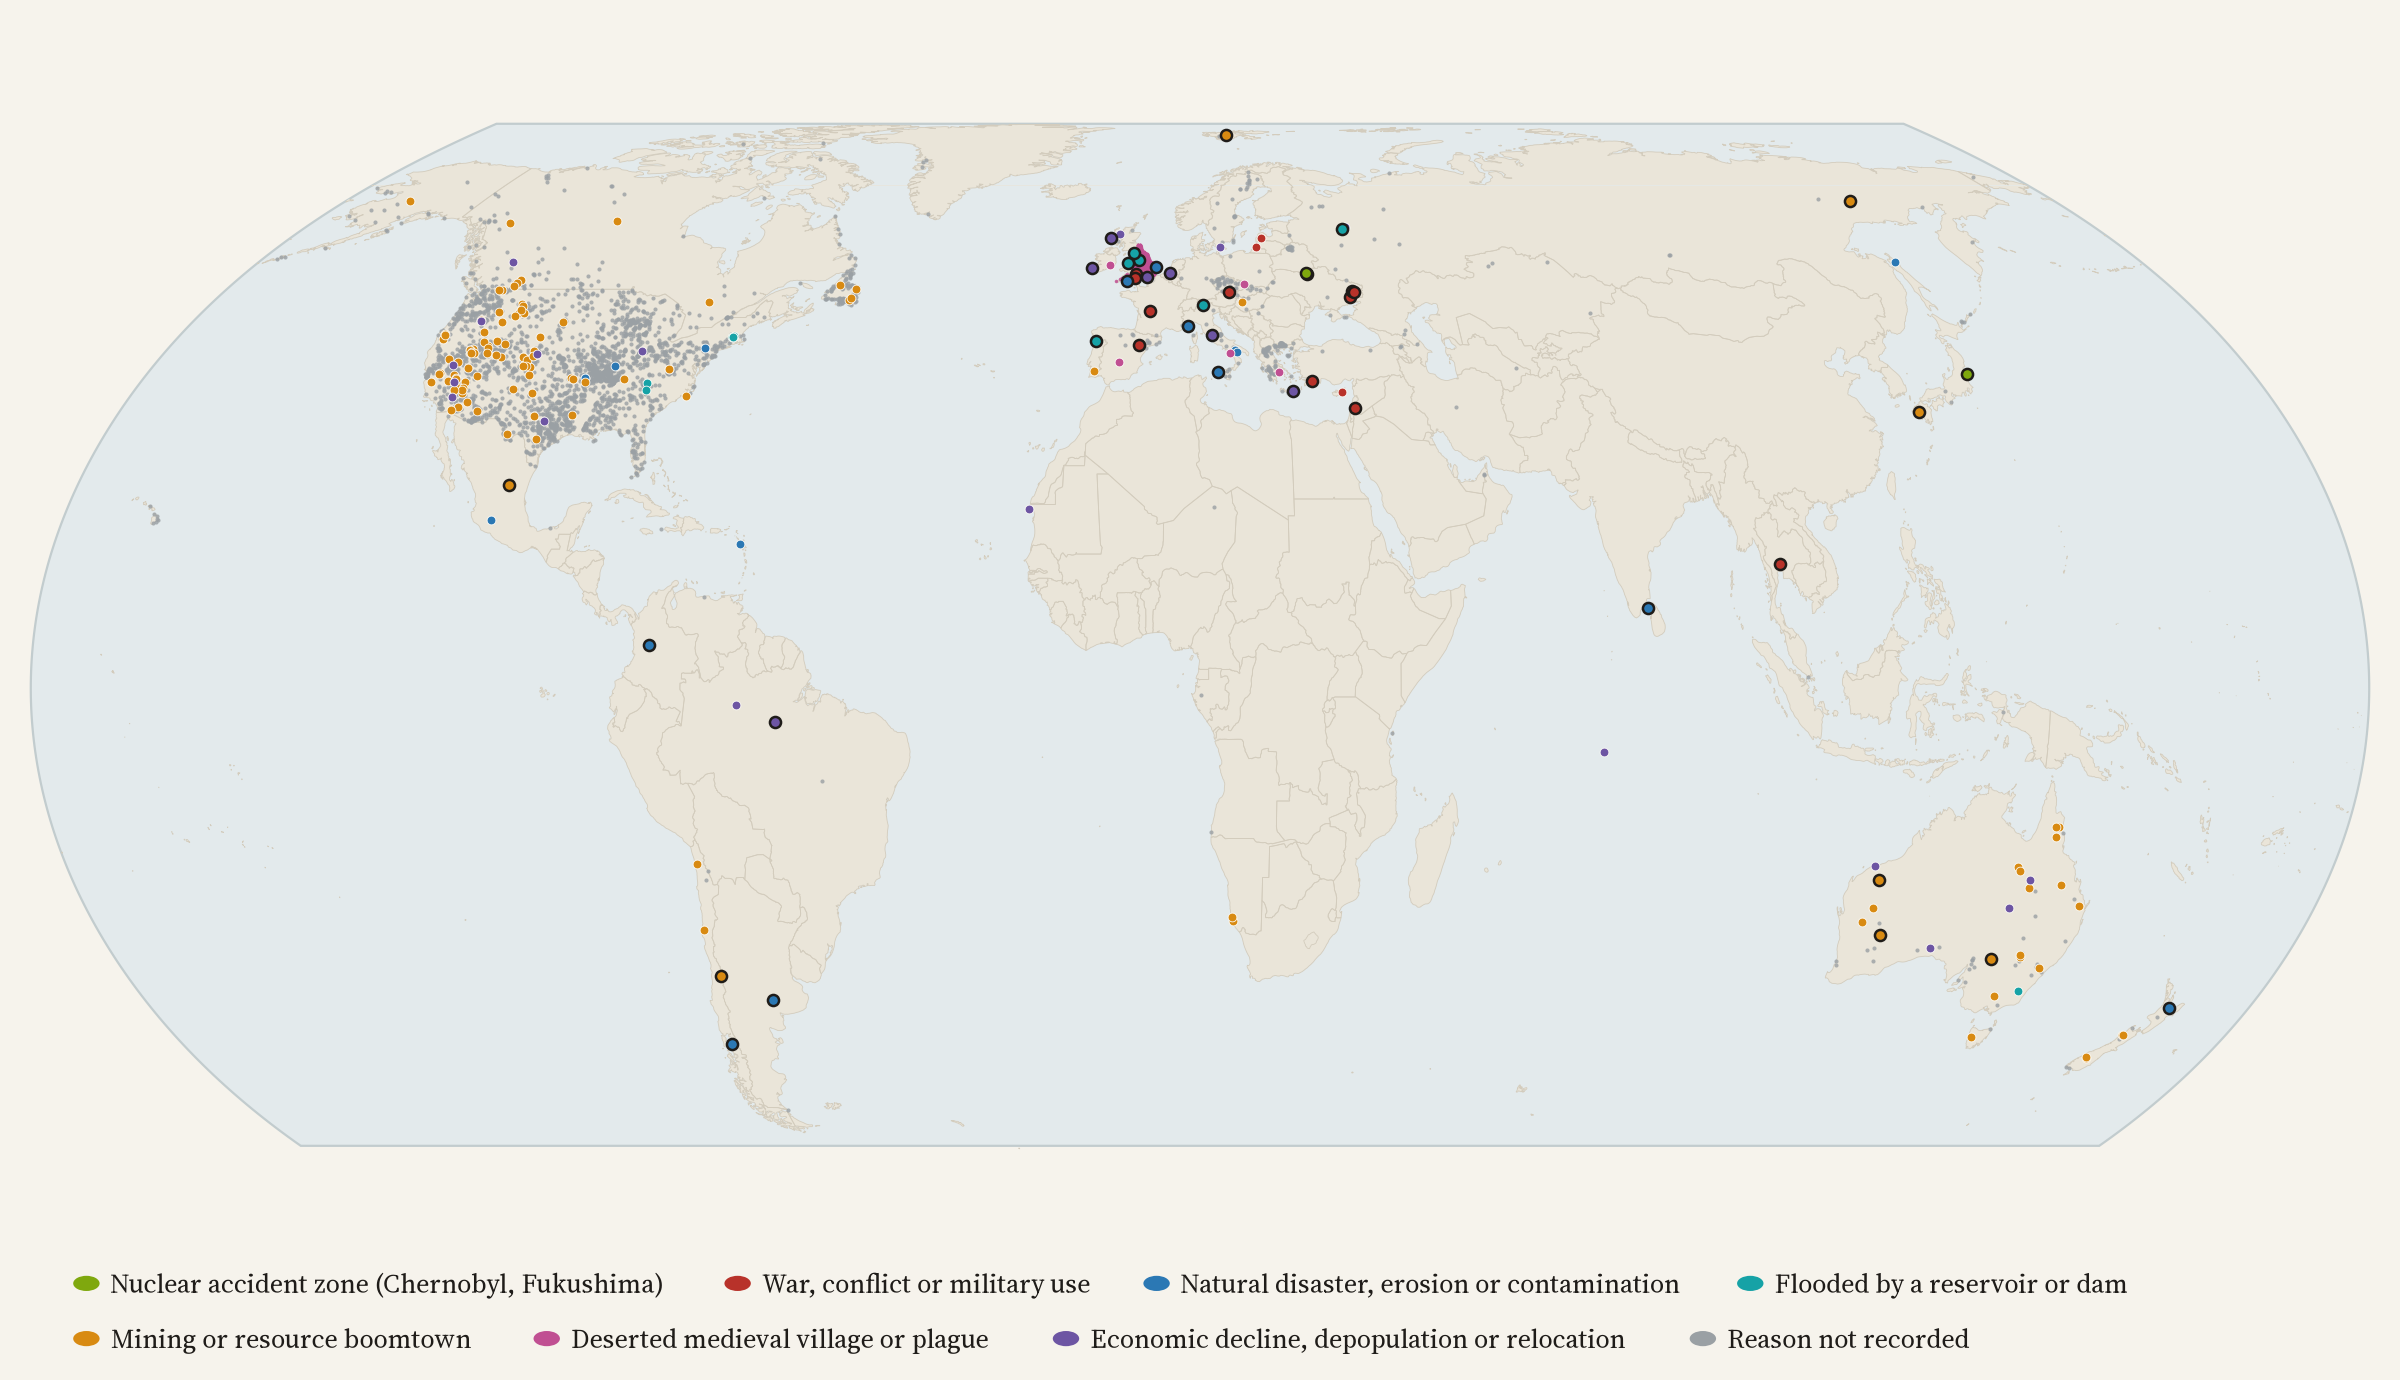
\includegraphics[width=\textwidth]{f_world.png}\caption{Abandoned settlements by reason: Wikidata ghost towns (small grey: reason not recorded), England's deserted medieval villages (magenta) and well-known places from Wikipedia's list placed by hand (ringed). Equal Earth projection.}\label{fig:world}\end{figure}

\begin{figure}[tbp]\centering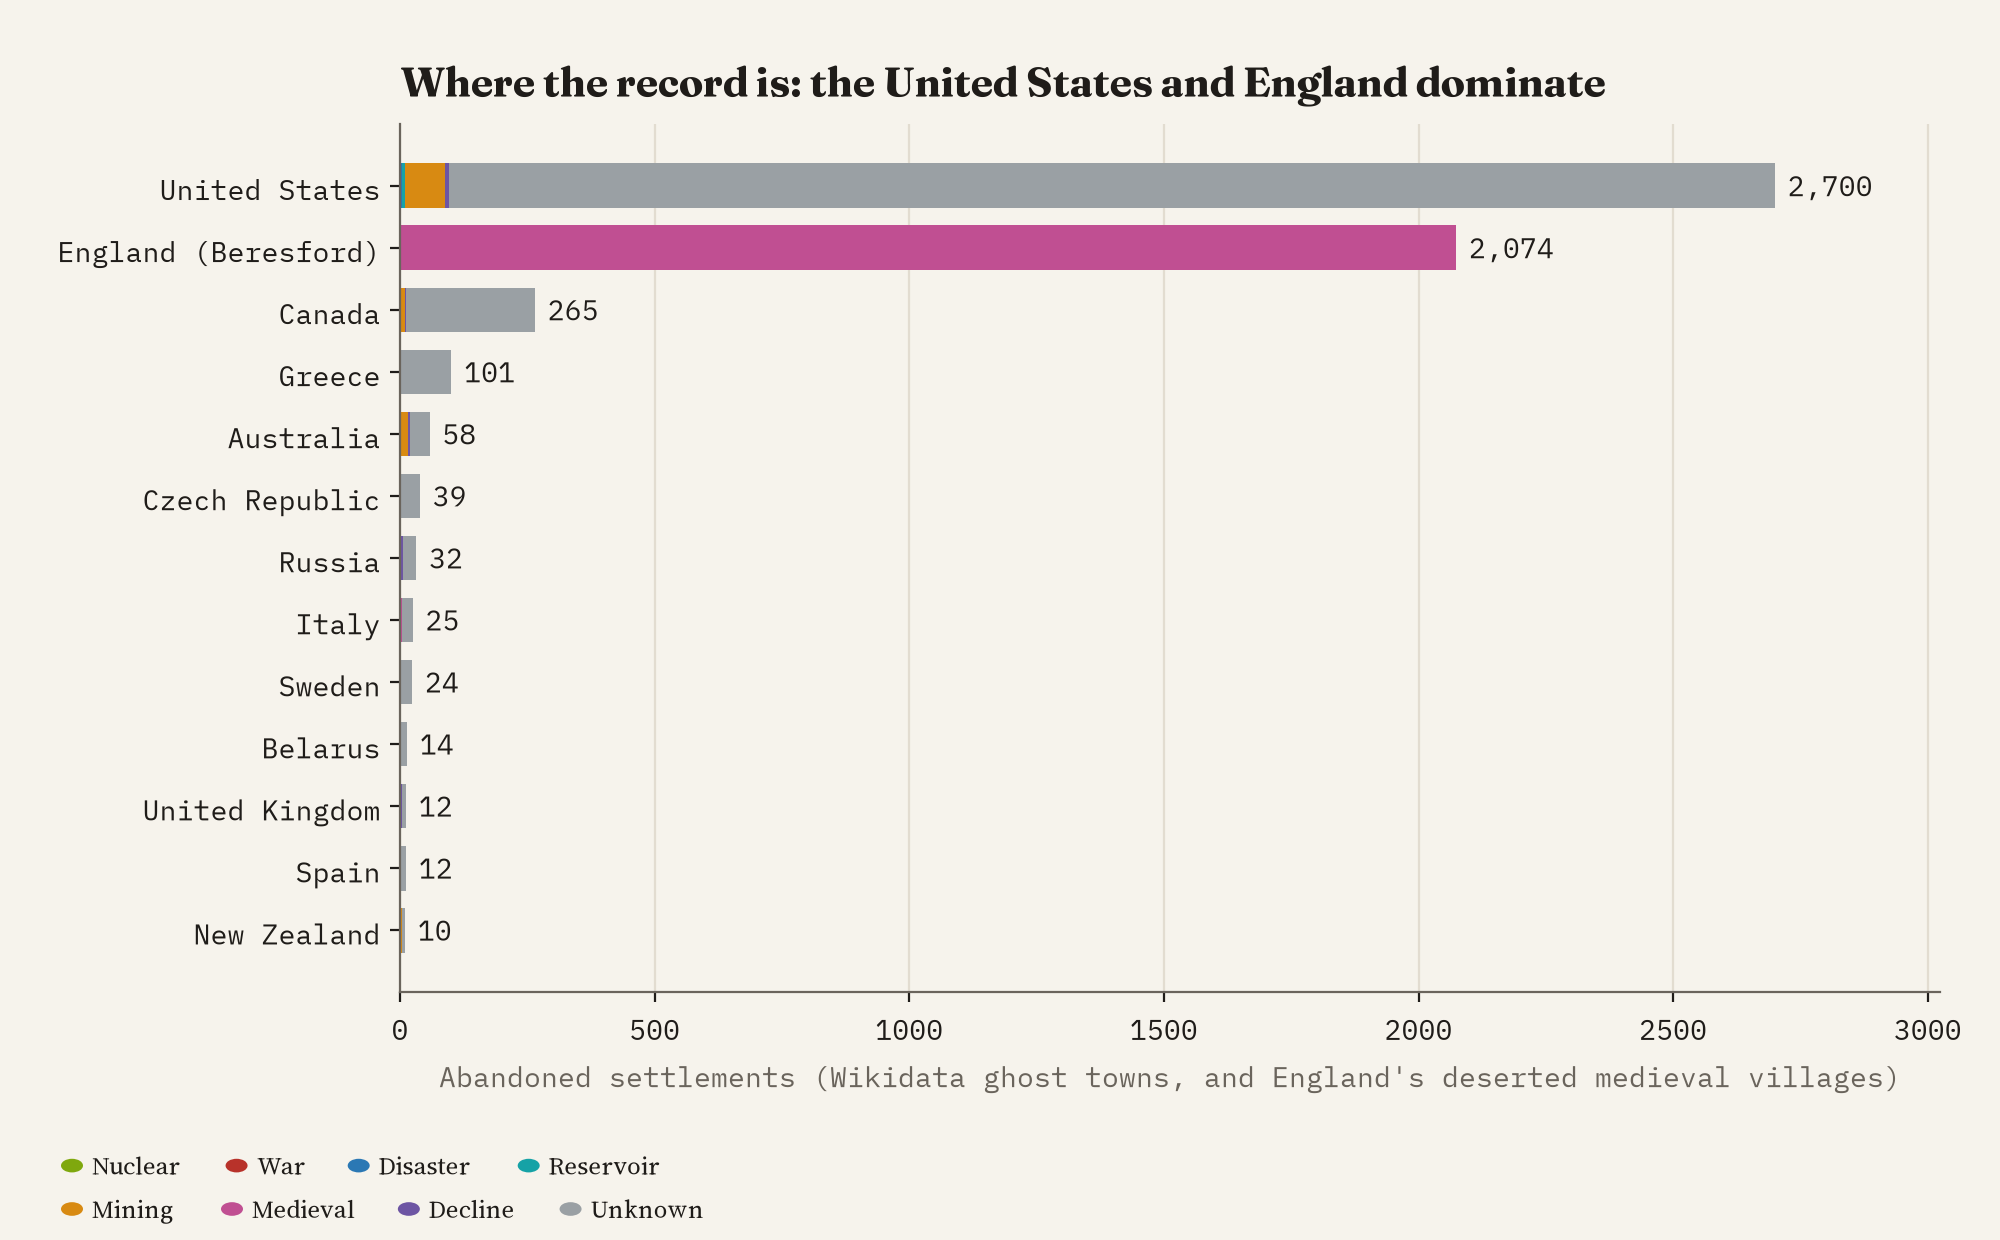
\includegraphics[width=\textwidth]{f_countries.png}\caption{Abandoned settlements by country and reason, with England's deserted medieval villages as a row of their own.}\label{fig:countries}\end{figure}

\subsection{How often the record says why}
Only 165 Wikidata ghost towns (4.9\%) yield a reason: 88 with high confidence, 16 medium and 61 low (Figure~\ref{fig:known}). The high-confidence reasons come from Wikidata descriptions (37), matched Wikipedia list entries (32), article sentences (16) and the Chernobyl zone (3). Of the ancient sites, 34 yield a reason. Wikipedia's list is far richer: 300 of 492 entries (61\%) give one.

\begin{figure}[tbp]\centering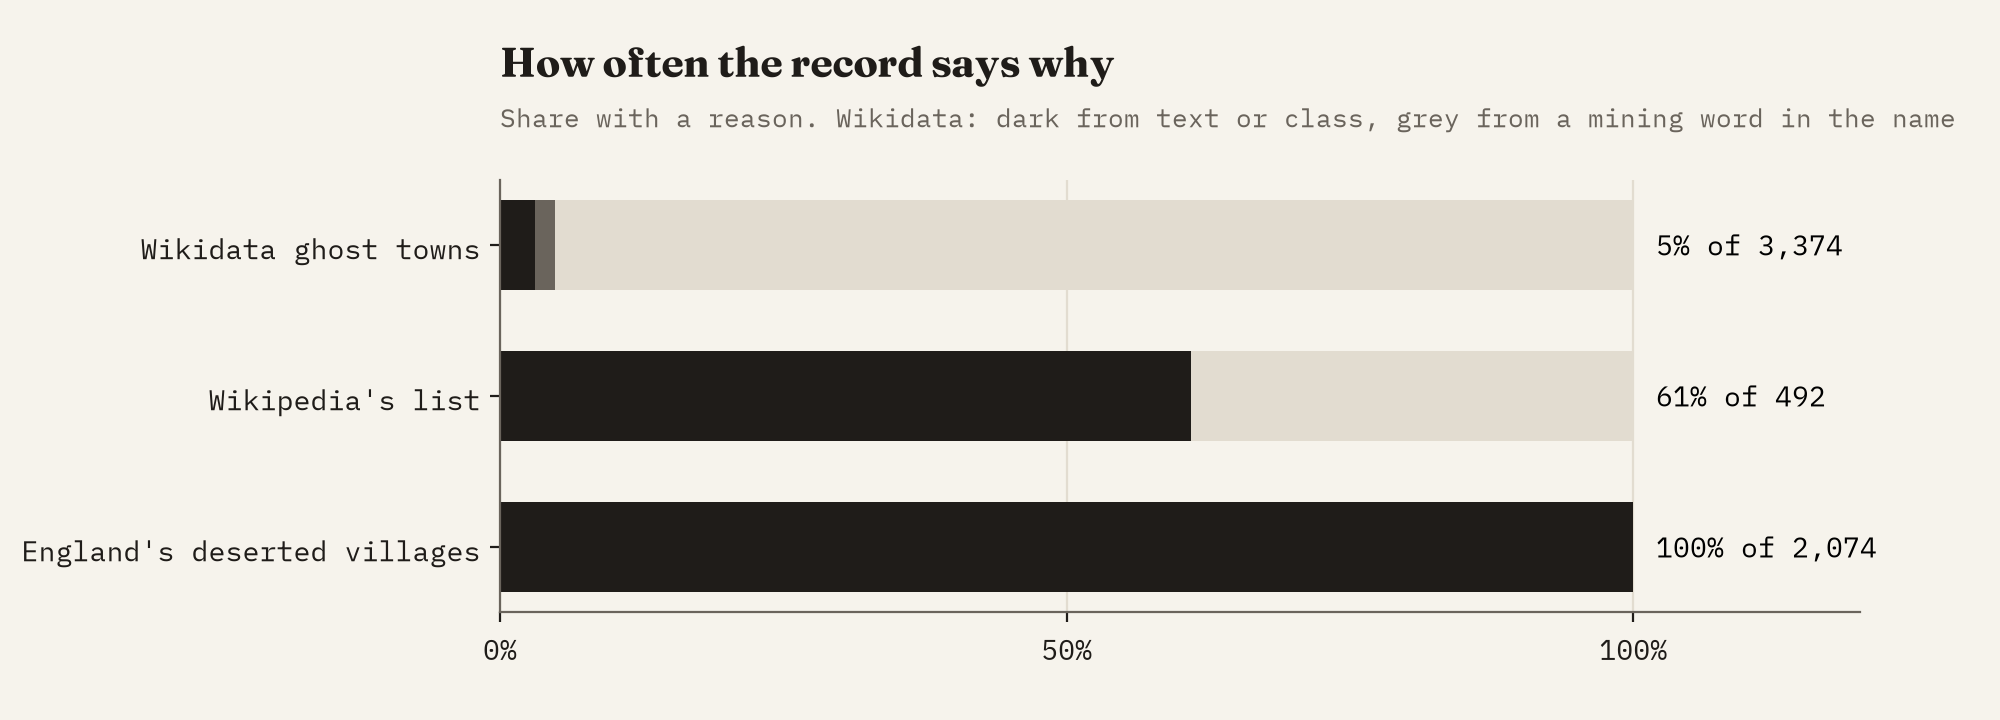
\includegraphics[width=0.85\textwidth]{f_known.png}\caption{Share of places with a reason in each source.}\label{fig:known}\end{figure}

\subsection{Why places were abandoned}
Across Wikipedia's list, mining and resource booms are the most common reason (81 entries), followed by war or military use (55), natural disasters and contamination (54), economic decline and depopulation (50), reservoirs (27), nuclear accidents (24) and medieval desertion (9). The mix differs by continent (Figure~\ref{fig:continents}). Mining dominates Oceania (41 of 69; 33 of 51 Australian entries) and Africa (11 of 29). Europe's 242 entries are the most varied, led by war (33), with the Chernobyl zone (23) and reservoirs (16). Mexico's 23 entries are split between reservoirs (8) and mining (8); the United Kingdom's 38 include 9 villages taken for military training, 6 lost to reservoirs and 5 to the sea or storms.

\begin{figure}[tbp]\centering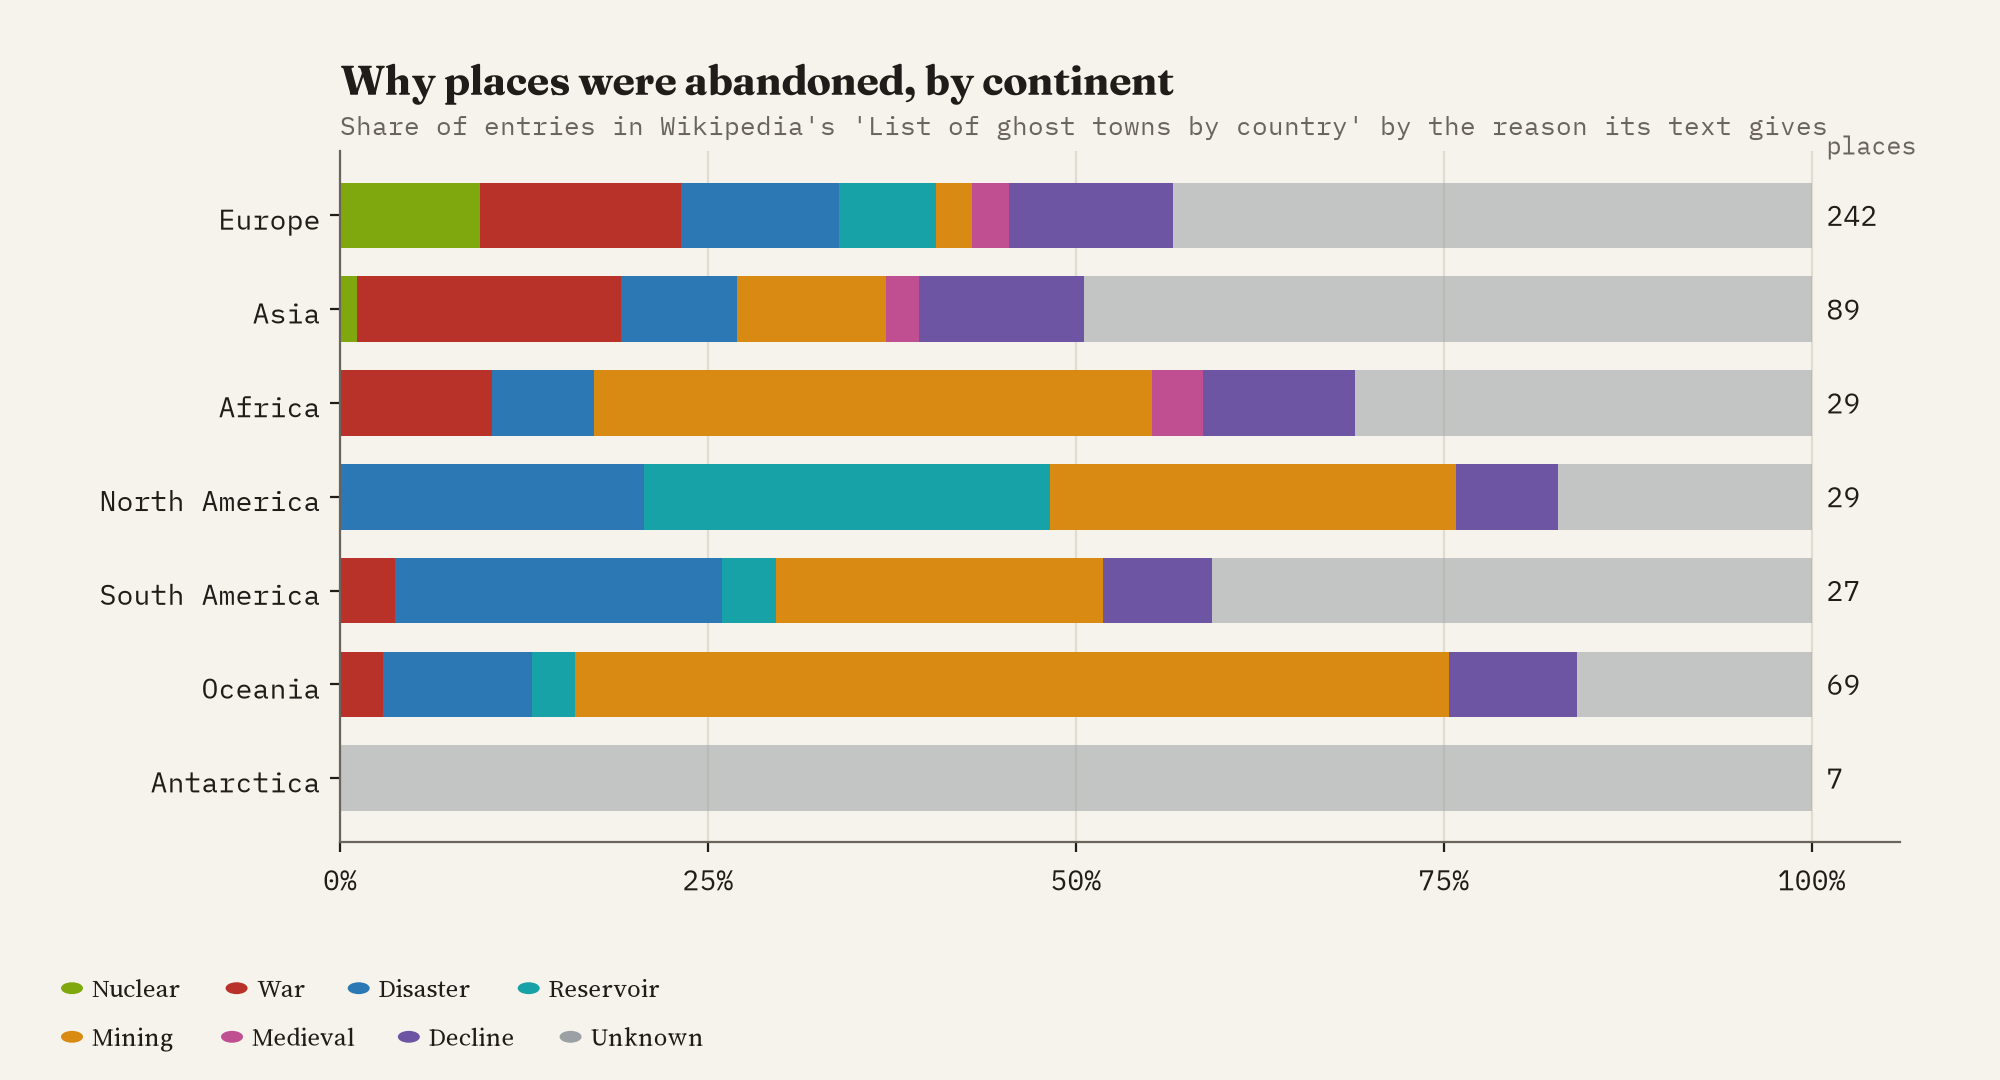
\includegraphics[width=\textwidth]{f_continents.png}\caption{Reasons in Wikipedia's `List of ghost towns by country', by continent (share of entries). North America excludes the United States and Canada.}\label{fig:continents}\end{figure}

\subsection{The American West}
1,053 of the American ghost towns (39\%) lie in the 11 western states, with Nevada (200) the most among them, but Texas (335) and Missouri (289) lead the country (Figure~\ref{fig:us}). Per area the West (3.4 per 10,000 km\textsuperscript{2}) and the rest of the contiguous country (3.3) are much alike. 65 western ghost towns are tied to mining (6.2\%), against 14 elsewhere (0.9\%), but only 18 of the western ones rest on text or class; 47 rest on names alone, and famous mining camps such as Bodie, California, and Rhyolite, Nevada, have no reason recorded. The data support the image of the mining West only weakly.

\begin{figure}[tbp]\centering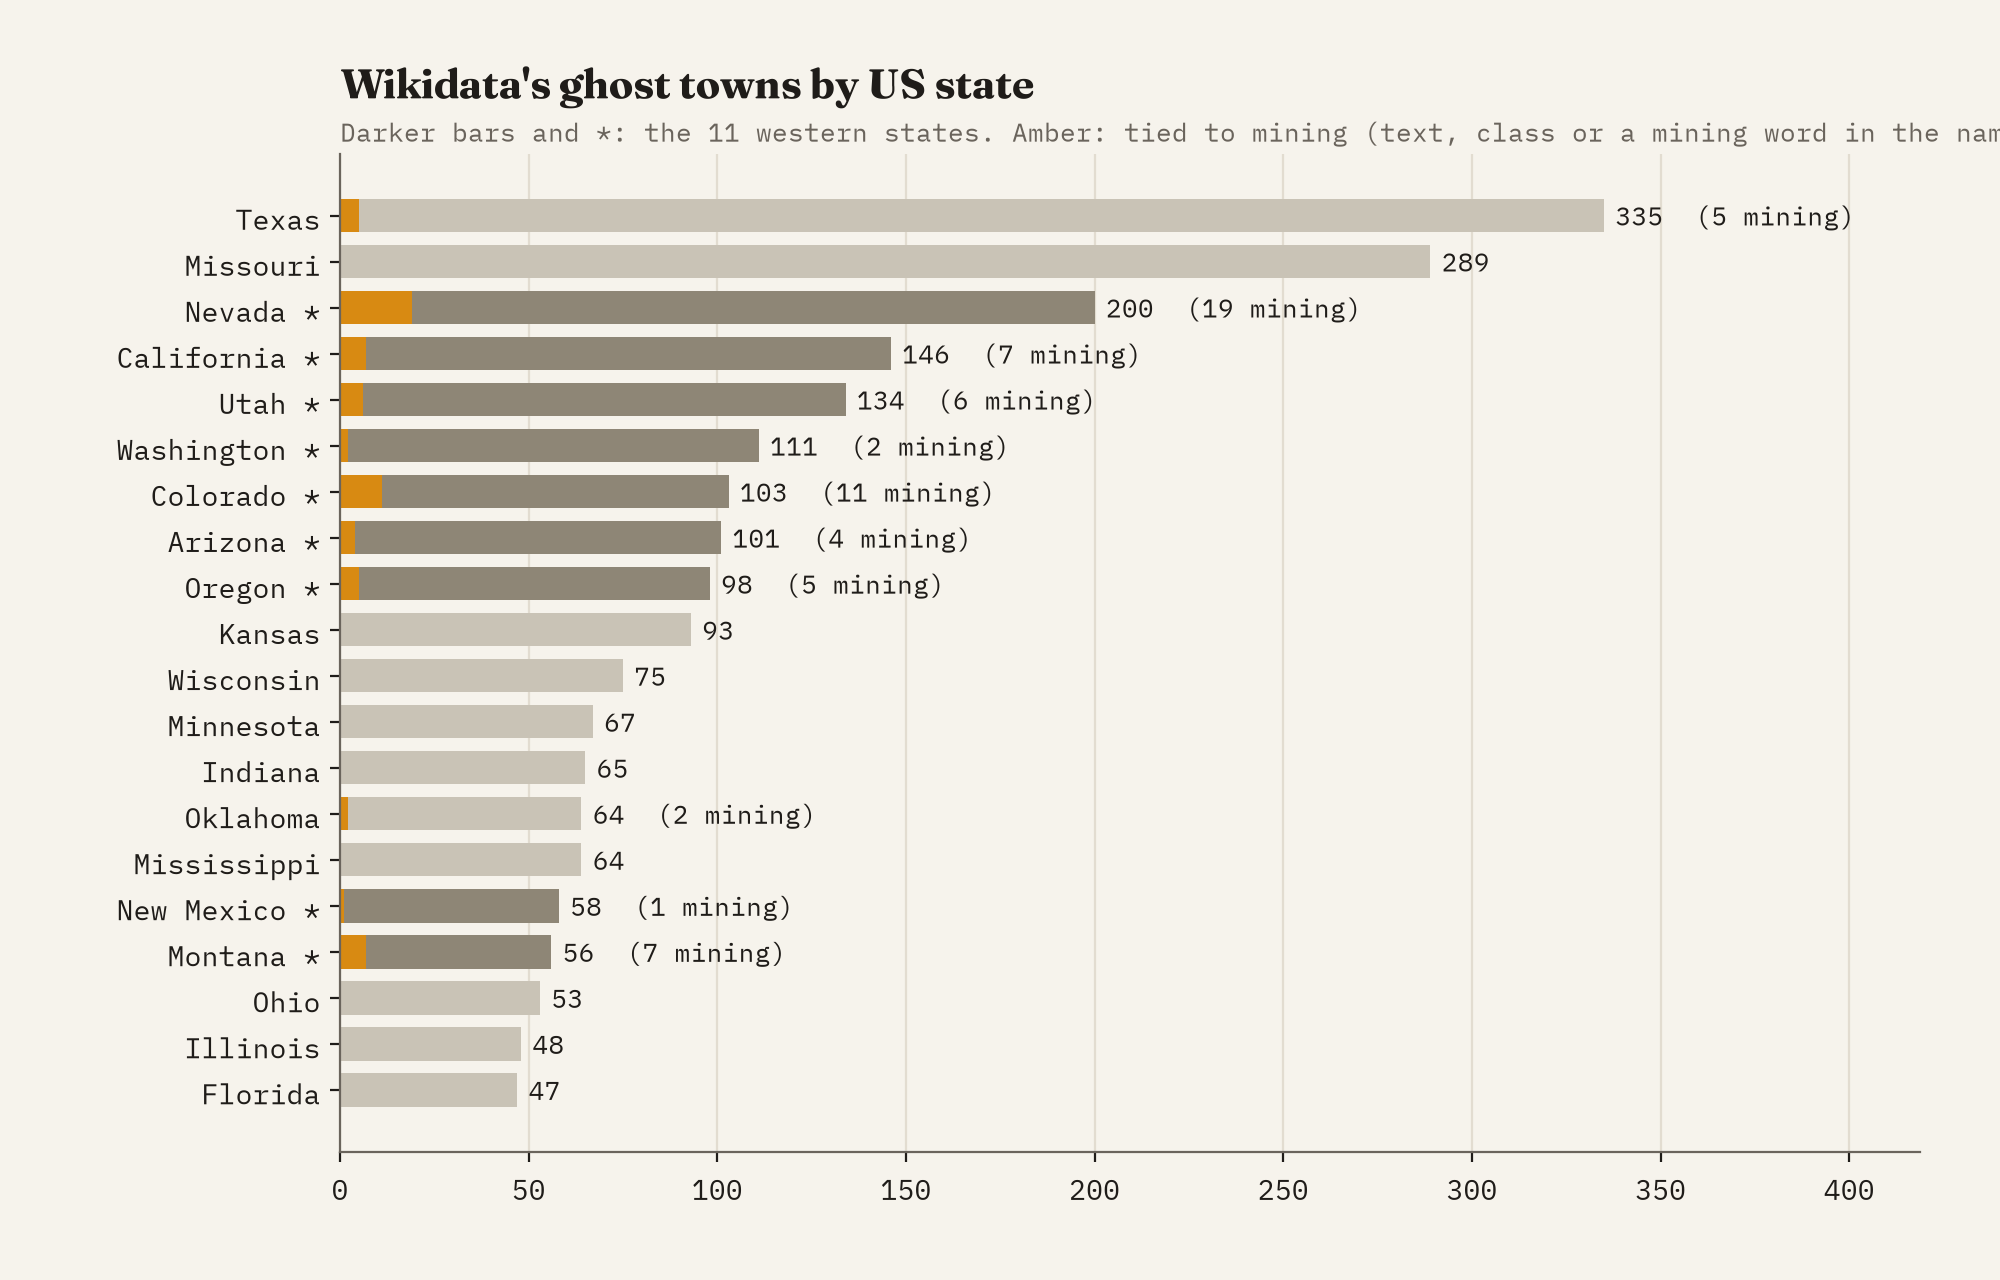
\includegraphics[width=\textwidth]{f_us_states.png}\caption{Wikidata ghost towns in the 20 US states with most; western states darker, mining in amber.}\label{fig:us}\end{figure}

\subsection{England's deserted medieval villages}
Beresford's gazetteer places 2,074 deserted villages and hamlets in 37 historic counties, 36\% of them in Yorkshire (358), Lincolnshire (220) and Northumberland (165) (Figure~\ref{fig:england}). Of 270 sites with a usable date, 17\% fall in 1348 to 1449, the century after the Black Death, and 59\% in 1450 to 1699, the age of enclosure and conversion to pasture. The written accounts mention enclosure or pasture 63 times, emparking 46, a monastic landholder 41, plague 32 and the sea or flooding 11, in line with \citet{beresfordhurst1971} and \citet{dyer2010}. Wikidata, by contrast, holds 2 ghost towns in England.

\begin{figure}[tbp]\centering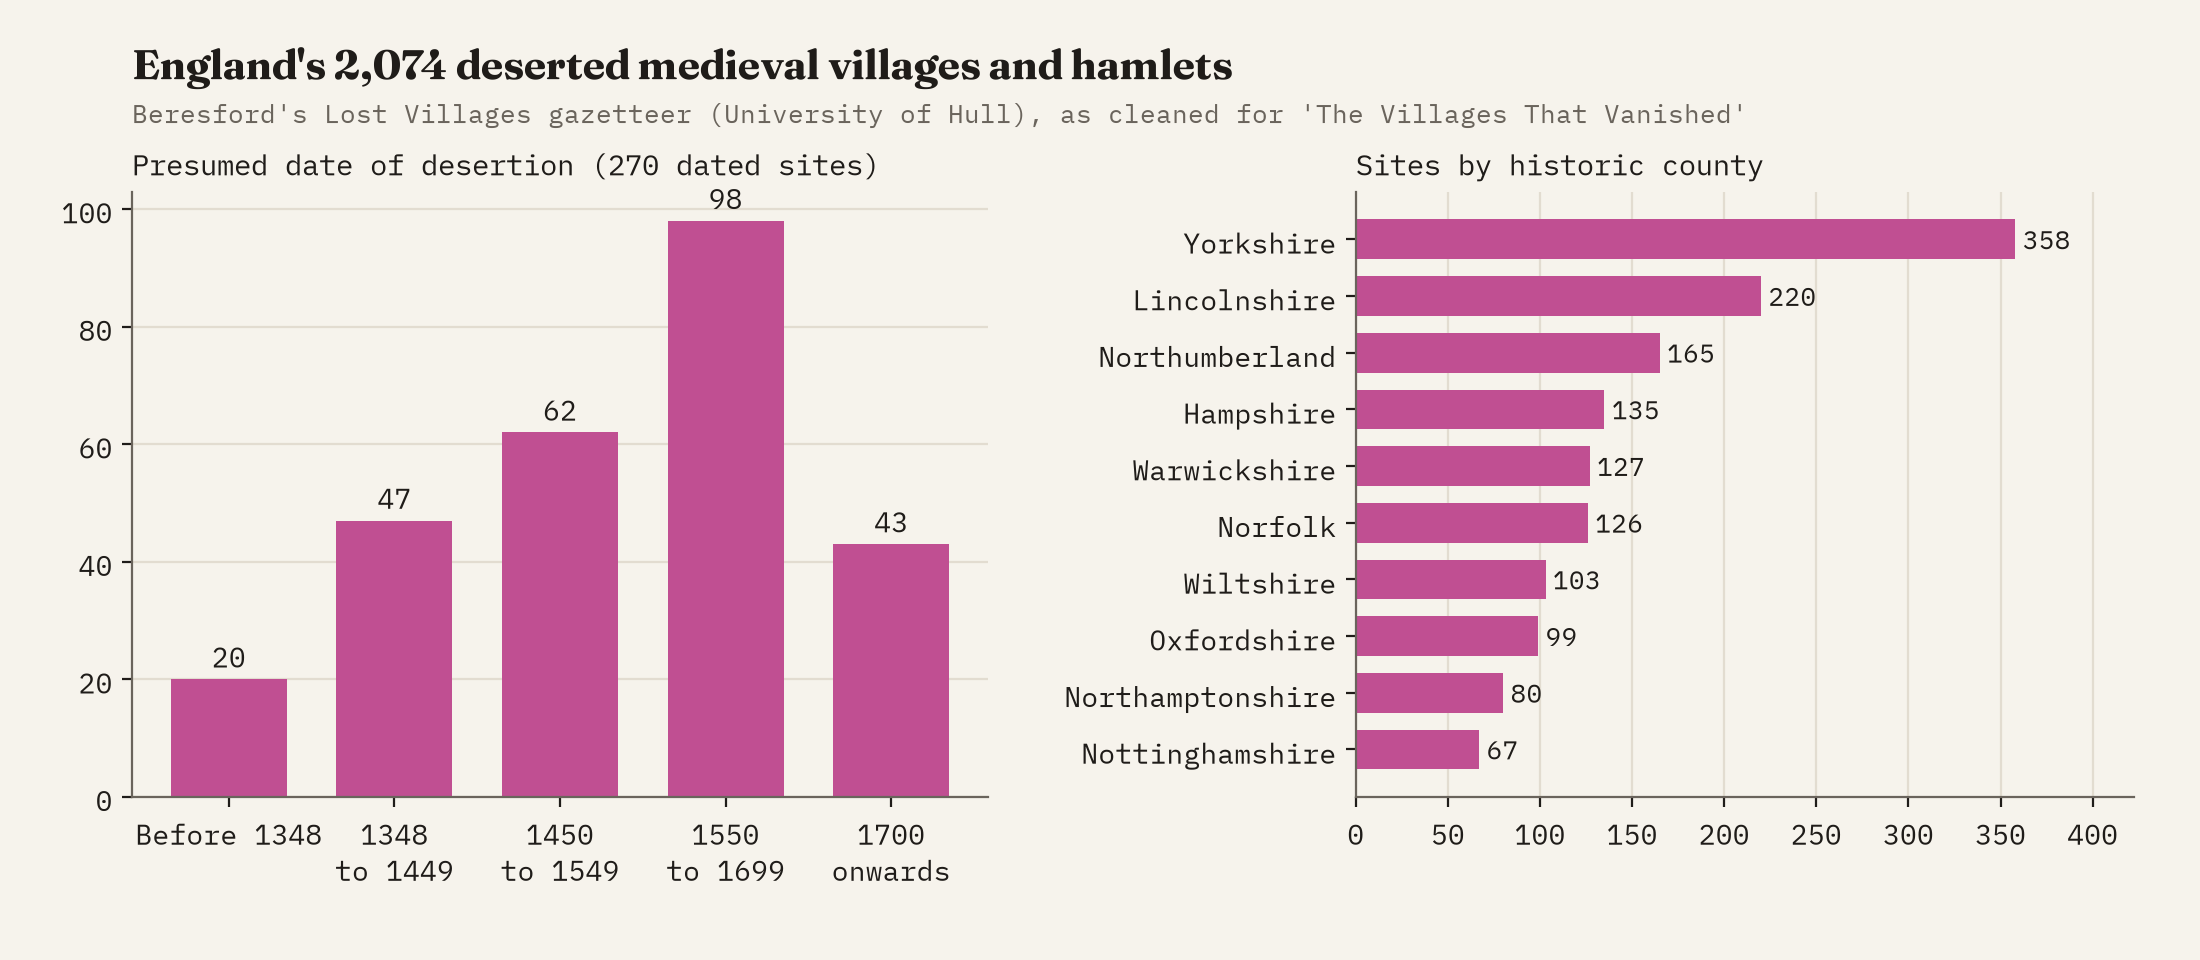
\includegraphics[width=\textwidth]{f_england.png}\caption{England's deserted medieval villages: presumed period of desertion and sites by historic county.}\label{fig:england}\end{figure}

\subsection{Soviet and post-Soviet abandonment}
The 15 former Soviet republics have 62 Wikidata ghost towns (32 in Russia, 14 in Belarus), 30 without an English name and 10 with a reason. Wikipedia's list has 82 entries in 12 of them (Figure~\ref{fig:soviet}). The largest group is the Chernobyl evacuation: 23 entries in Ukraine and Belarus. Others are resource and military towns of the Soviet period (Kadykchan, Khalmer-Yu, Butugychag, Chagan, Skrunda-1), 10 depopulated or abandoned villages in Yaroslavl Oblast, where the town of Mologa was flooded for the Rybinsk Reservoir, and 7 Ukrainian towns emptied by fighting since 2022. Tajikistan's 15 entries, abandoned villages mostly in the Ayni District, come with a note that the cause is unknown.

\begin{figure}[tbp]\centering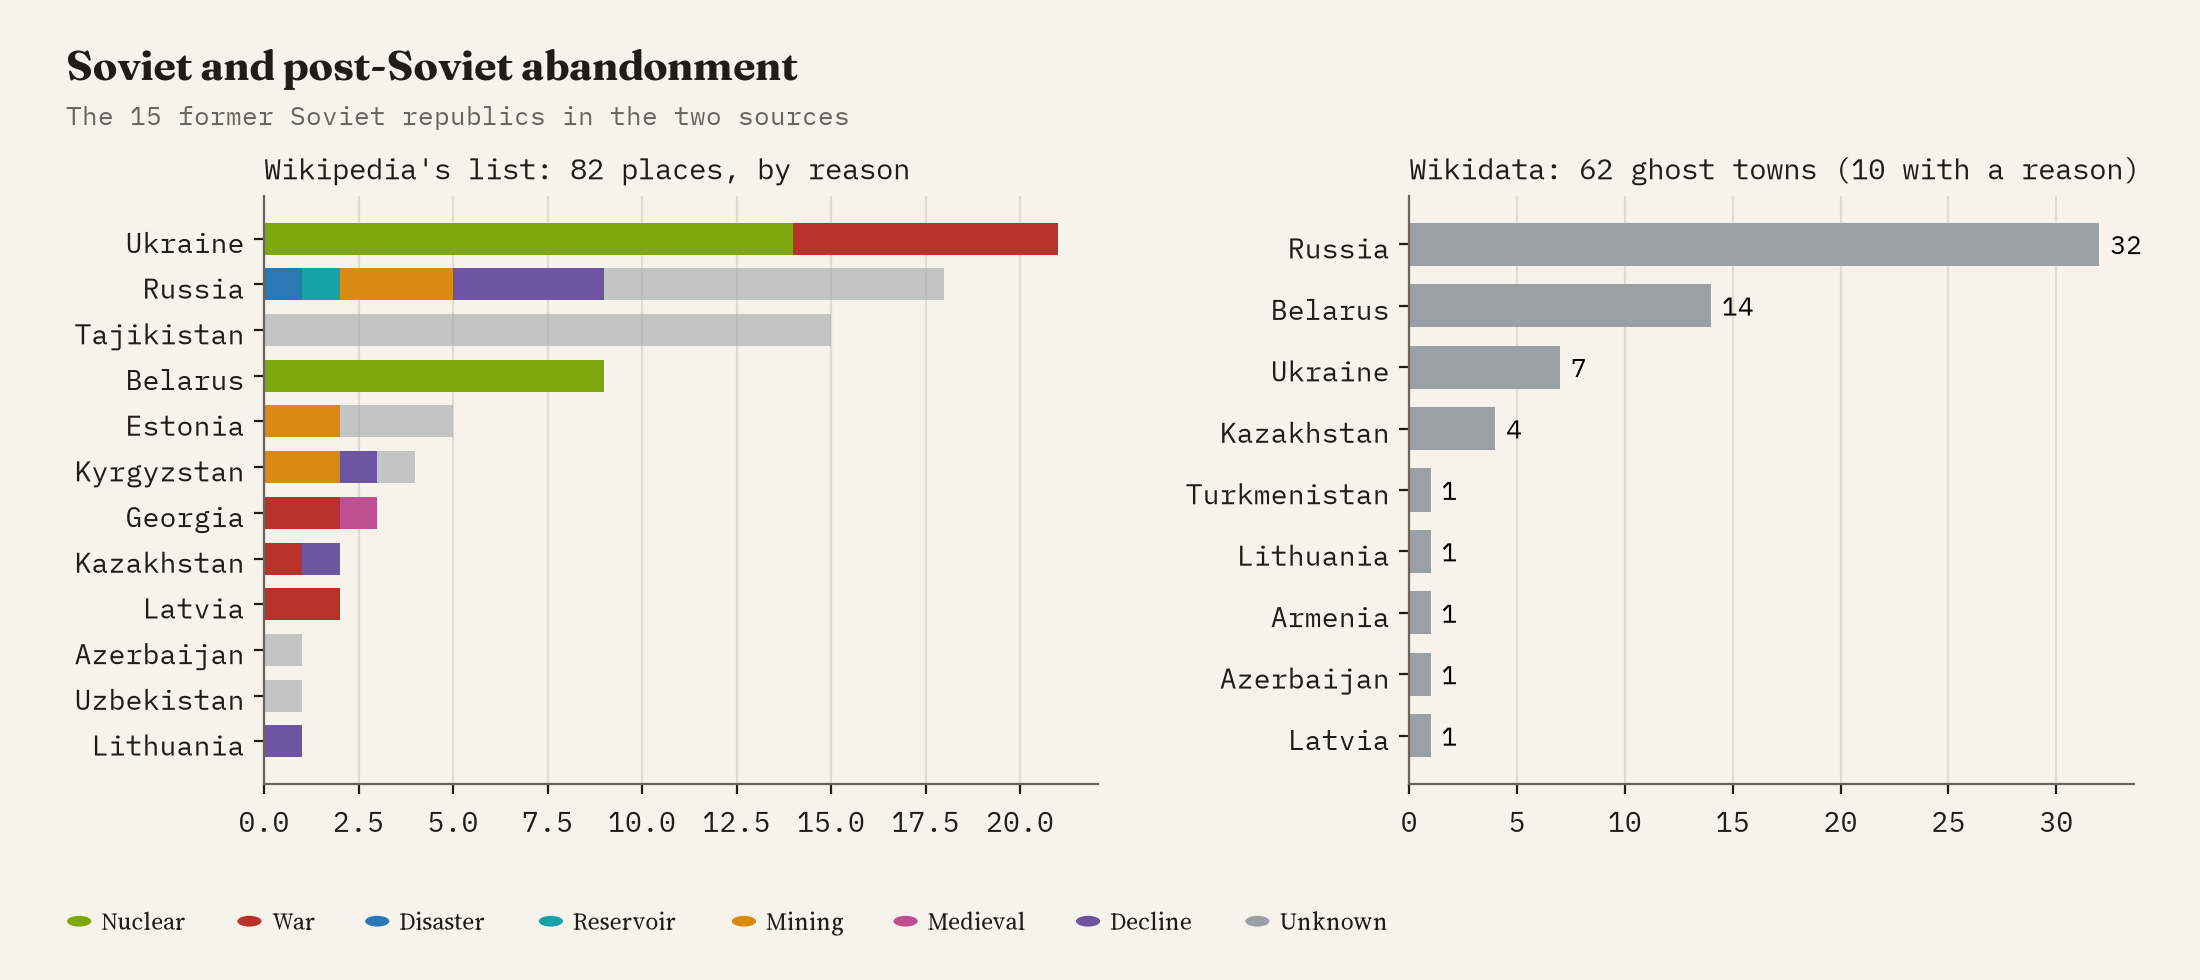
\includegraphics[width=\textwidth]{f_soviet.png}\caption{Post-Soviet places: Wikipedia list entries by reason (left) and Wikidata ghost towns by country (right).}\label{fig:soviet}\end{figure}

\subsection{When}
Wikidata's 46 dissolution dates range from 1420 to 2020, 36 of them after 1900. Of the 156 dated Wikipedia entries, 85\% fall after 1900 and 33 after 2000 (Figure~\ref{fig:when}). The busiest decades are the 2010s (19), the 1980s (17, with Chernobyl) and the 1950s (16). The median year is 1951 for reservoirs and 1953 for mining towns. England's dated deserted villages, centred on 1550, are the only large body of early dates.

\begin{figure}[tbp]\centering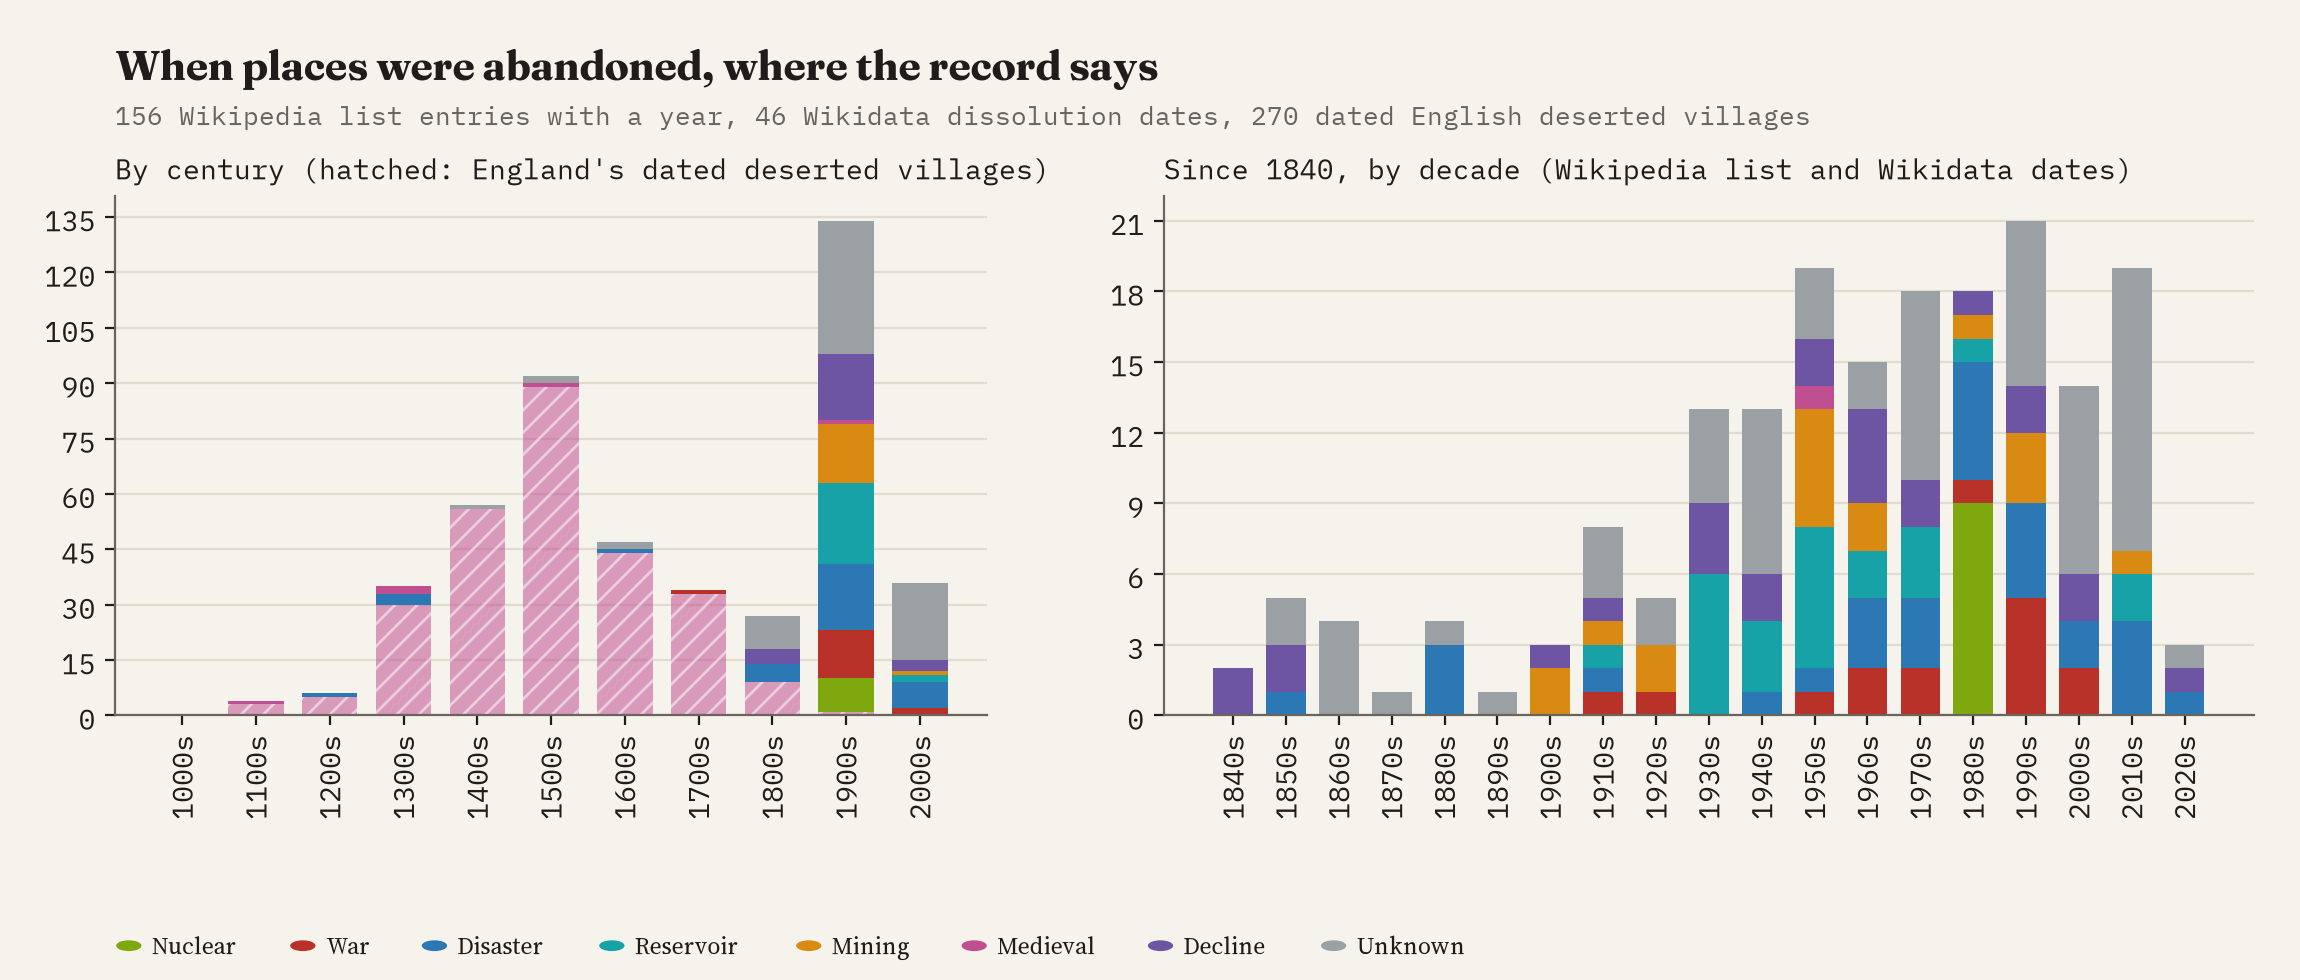
\includegraphics[width=\textwidth]{f_when.png}\caption{Dated abandonments by century (left; hatched: England's deserted villages) and by decade since 1840 (right), coloured by reason.}\label{fig:when}\end{figure}

\section{Limitations}
The map shows the record, not history. The United States and England dominate because of bulk imports into Wikidata and seventy years of scholarship on English villages; most of Africa, Asia and South America is nearly blank, and the Wikidata class tree both includes living places (removed here) and misses famous ghost towns filed under other classes. Reasons come from keyword rules on short texts and can be wrong: a word can mislead, the priority order picks one of several causes, and names are weak evidence. Wikipedia's list is a selection of notable places, edited by many hands, not a sample. Hand-placed positions are approximate. Dates are scarce and uneven. The classification of England's deserted villages under one heading hides their real variety of causes. Some places counted as ghost towns still have small populations.

\section*{Data availability}
Code and derived data are at \url{https://github.com/Tristan-Hotham/ghost-towns} and archived with this paper at \url{https://doi.org/10.5281/zenodo.23857616}. The Wikidata-derived table is CC BY 4.0; tables containing Wikipedia text are CC BY-SA 4.0; the England table, derived from Beresford's Lost Villages, is CC BY-NC-SA 4.0, as are this text and the figures; the code is MIT licensed. The interactive map is at \url{https://maps.tristanhotham.com/ghost-towns/}.

\section*{AI statement}
I wrote the text, with drafting and editing assistance from Claude (Anthropic), which also helped prepare the analysis code. I reviewed and checked all text and results.

\begin{thebibliography}{99}
\bibitem[Beresford(1954)]{beresford1954} Beresford, M. (1954) \emph{The Lost Villages of England}. London: Lutterworth Press.
\bibitem[Beresford and Hurst(1971)]{beresfordhurst1971} Beresford, M. and Hurst, J.G. (eds.) (1971) \emph{Deserted Medieval Villages: Studies}. London: Lutterworth Press. Gazetteer online as Beresford's Lost Villages, University of Hull, \url{https://dmv.wordpress.hull.ac.uk/}, CC BY-NC-SA 4.0.
\bibitem[Dyer and Jones(2010)]{dyer2010} Dyer, C. and Jones, R. (eds.) (2010) \emph{Deserted Villages Revisited}. Hatfield: University of Hertfordshire Press.
\bibitem[Hotham(2026)]{hotham2026lv} Hotham, T. (2026) The Villages That Vanished: England's deserted medieval villages, Domesday Book and the record of desertion. Zenodo. \url{https://doi.org/10.5281/zenodo.23677161}
\bibitem[Natural Earth(2026)]{naturalearth} Natural Earth (2026) 1:10m and 1:50m cultural and physical vectors. Public domain. \url{https://www.naturalearthdata.com/}
\bibitem[Paul(1963)]{paul1963} Paul, R.W. (1963) \emph{Mining Frontiers of the Far West, 1848 to 1880}. New York: Holt, Rinehart and Winston.
\bibitem[Wikidata(2026)]{wikidata} Wikidata (2026) Items classed as ghost town (Q74047), abandoned village (Q15661340) or deserted medieval village (Q1952852), queried via QLever. CC0. \url{https://www.wikidata.org/}
\bibitem[Wikipedia(2026a)]{wikighost} Wikipedia contributors (2026a) Ghost town. \emph{English Wikipedia}. CC BY-SA 4.0. \url{https://en.wikipedia.org/wiki/Ghost_town}
\bibitem[Wikipedia(2026b)]{wikilist} Wikipedia contributors (2026b) List of ghost towns by country. \emph{English Wikipedia}. CC BY-SA 4.0. \url{https://en.wikipedia.org/wiki/List_of_ghost_towns_by_country}
\end{thebibliography}
\end{document}
